\documentclass{article}
\usepackage[english,russian]{babel}
\usepackage{textcomp}
\usepackage{geometry}
  \geometry{left=2cm}
  \geometry{right=1.5cm}
  \geometry{top=1.5cm}
  \geometry{bottom=2cm}
\usepackage{tikz}
\usepackage{multicol}
\usepackage{listings}
\pagenumbering{gobble}

\lstdefinestyle{csMiptCppStyle}{
  language=C++,
  basicstyle=\linespread{1.1}\ttfamily,
  columns=fixed,
  fontadjust=true,
  basewidth=0.5em,
  keywordstyle=\color{blue}\bfseries,
  commentstyle=\color{gray},
  texcl=true,
  stringstyle=\ttfamily\color{orange!50!black},
  showstringspaces=false,
  %numbers=false,
  numbersep=5pt,
  numberstyle=\tiny\color{black},
  numberfirstline=true,
  stepnumber=1,      
  numbersep=10pt,
  backgroundcolor=\color{white},
  showstringspaces=false,
  captionpos=b,
  breaklines=true
  breakatwhitespace=true,
  xleftmargin=.2in,
  extendedchars=\true,
  keepspaces = true,
  tabsize=4,
  upquote=true,
}
\lstdefinestyle{csMiptCppBorderStyle}{
  style=csMiptCppStyle,
  framexleftmargin=5mm, 
  frame=shadowbox, 
  rulesepcolor=\color{gray}
}

\lstset{style=csMiptCppStyle}
\lstset{literate={~}{{\raisebox{0.5ex}{\texttildelow}}}{1}}


\begin{document}
\title{Семинар \#2: Наследование. \vspace{-5ex}}\date{}\maketitle
Наследование (англ. \textit{inheritance}) -- это концепция объектно-ориентированного программирования, согласно которой абстрактный тип данных может наследовать данные и функциональность некоторого существующего типа, способствуя повторному использованию компонентов программного обеспечения.

Наследование в C++ позволяет создавать классы на основе уже существующих классов. Класс от которого происходит наследование принято называть \textit{базовым}, \textit{родительским} или \textit{суперклассом}, в то время как класс, который наследует от него, именуется \textit{производным}, \textit{дочерним} или \textit{подклассом}. Всё это эквивалентные определения. В английском языке используются аналогичные термины \textit{base}/\textit{derived}, \textit{parent}/\textit{child} и \textit{superclass}/\textit{subclass}. Производный класс наследует от базового класса его поля и методы и может пользоваться ими. Наследование также применимо и к структурам, так как классы и структуры в C++ почти ничем не отличаются.

Рассмотрим пример в котором есть базовый класс \texttt{Alice} и производный класс \texttt{Bob}. То от какого класса наследуется данный класс, прописывается в определении класса через двоеточие. В этом примере класс \texttt{Bob} наследует от класса \texttt{Alice} поле \texttt{apple} и метод \texttt{ask} и может их использовать.
\begin{lstlisting}
#include <iostream>
struct Alice
{
    int apple = 10;
    void ask() {std::cout << "ask" << std::endl;}
};

struct Bob : Alice
{
    int banana = 20;
    void buy() {std::cout << "buy" << std::endl;}
};

int main()
{
    Bob b;
    std::cout << b.apple << " " << b.banana << std::endl;
    b.ask();
    b.buy();
}
\end{lstlisting}
Зависимомость между классами \texttt{Alice} и \texttt{Bob} часто представляют в виде следующей диаграммы:
\begin{center}
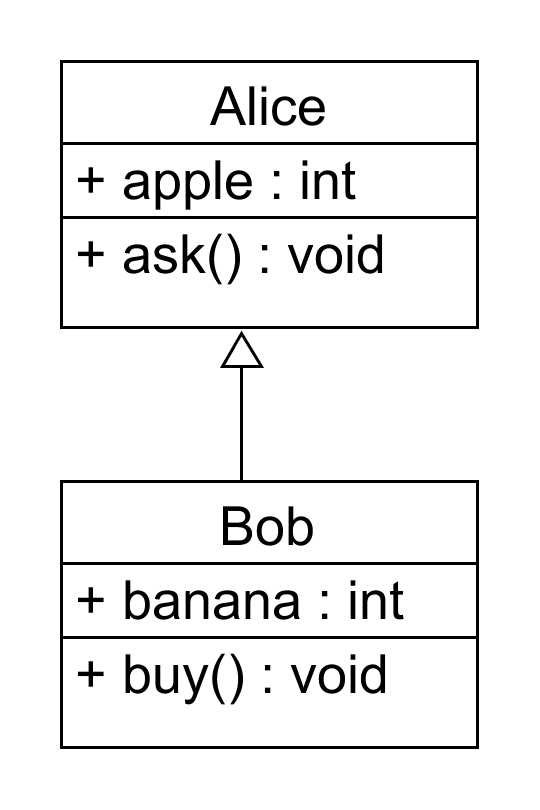
\includegraphics[scale=0.18]{../images/alice_bob.png}
\end{center}
Это так называемая UML Class диаграмма. Наследование на такой диаграмме обозначается стрелкой с полым треугольным наконечником. Направлена стрелки -- от производного класса к базовому. Знак плюс перед членами класса означает, что они публичные.

В памяти классы \texttt{Alice} и \texttt{Bob} можно представить следующим образом:
\begin{center}
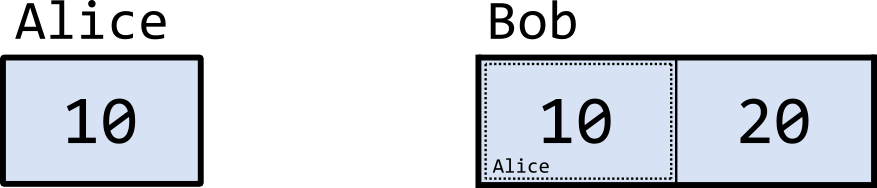
\includegraphics[scale=1]{../images/alice_bob_in_memory.png}
\end{center}
Производный класс \texttt{Bob} будет содержать внутри себя объект базового класса \texttt{Alice}. Это полностью корректный объект базового класса. Даже если создать указатель типа \texttt{Alice*}, указать им на объект типа \texttt{Bob} и разыменовать, то это будет корректно и в результате разыменования получится объект типа \texttt{Alice}, хранящийся внутри \texttt{Bob}.


\section*{Примеры наследования}




\section*{Затенение членов базового класса}
Название полей и методов в базовом и производном классах может совпадать. Это не приведёт к ошибке. В этом случае, члены базового класса будут \textit{затенены} членами производного класса. 
\begin{lstlisting}
#include <iostream>
struct Alice
{
	int x = 10;
	void func() {std::cout << "alice func" << std::endl;}
};

struct Bob : Alice
{
	int x = 20;
	void func() {std::cout << "bob func" << std::endl;}
};

int main()
{
	Bob b;
	std::cout << b.x << std::endl;          // Напечатает 20
	b.func();						        // Напечатает bob func
	
	std::cout << b.Alice::x << std::endl;   // Напечатает 10
	b.Alice::func();					    // Напечатает alice func
}
\end{lstlisting}
В этом случае получить доступ к членам базового класса можно с помощью специального синтаксиса:
\begin{lstlisting}
Bob b;
b.Alice::func(); // Вызываем затенённый метод базового класса Alice, 
				 // используя объект производного класса Bob
\end{lstlisting}
Eсли методы в родительском классе перегружены, то метод с тем же именем в дочернем классе затенит сразу все перегрузки родительского класса:
\begin{lstlisting}
#include <iostream>
struct Alice
{
	void func(float x)  {std::cout << "float" << std::endl;}
	void func(double x) {std::cout << "double" << std::endl;}
};

struct Bob : Alice
{
	void func(int x)    {std::cout << "int" << std::endl;}
};

int main()
{
	Bob b;
	b.func(1.5);         // Напечатает int, так cat из Bob затеняет все func из Alice
	b.Alice::func(1.5);  // Напечатает double, выбирает func из Alice по правилам перегрузки
}
\end{lstlisting}
Другими словами \texttt{Alice::func} и \texttt{Bob::func} это разные функции не являющиеся перегрузками друг друга.

Затенение в наследнике работает похожим образом на затенение в новой области видимости или в новом пространстве имён. Например, при работе с пространствами имён похожая ситуация выглядит так:
\begin{lstlisting}
#include <iostream>
void func(float x)   {std::cout << "float" << std::endl;}
void func(double x)  {std::cout << "double" << std::endl;}
namespace mipt
{
	void func(int x) {std::cout << "int" << std::endl;}
	void test() {func(1.5);} // func из mipt затеняет func из глобального пространства
}
int main()
{
	mipt::test();   // Напечатает int
	func(1.5);      // Напечатает double
}
\end{lstlisting} 

\newpage
\section*{Модификация доступа}

\subsection*{Защищённые члены класса. Модификатор доступа \texttt{protected}.}
Приватные члены класса доступны только в самом классе и в друзьях класса, но не в дочерних классах.\\
Защищённые члены класса доступны в самом классе, в друзьях и в дочерних классах.
\begin{lstlisting}
#include <iostream>
struct Alice
{
public:
	int x = 10;  // Публичное поле
protected:
	int y = 20;  // Защищённое поле
private:
	int z = 30;  // Приватное поле
};

struct Bob : Alice
{
	void func() 
	{
		std::cout << x << std::endl;  // ОК, доступ есть, так как поле x публичное
		std::cout << y << std::endl;  // ОК, доступ есть, так как поле y защищённое
		std::cout << z << std::endl;  // Ошибка, нет доступа к z, так как поле z приватное
	}  
};

int main()
{
	Alice a;
	std::cout << a.x << std::endl;  // ОК, доступ есть, так как поле x публичное
	std::cout << a.y << std::endl;  // Ошибка, нет доступа к y, так как поле y защищённое
	std::cout << a.z << std::endl;  // Ошибка, нет доступа к z, так как поле z приватное
}
\end{lstlisting}
Получать доступ к защищённому полю в производном классе можно только через объект производного класса:
\begin{lstlisting}
struct Alice
{
protected:
    int y = 20;
};

struct Bob : Alice
{
    void func(Alice& a, Bob& b) 
    {
        std::cout << y   << std::endl;  // ОК
        std::cout << a.y << std::endl;  // Ошибка
        std::cout << b.y << std::endl;  // ОК
    }  
};
\end{lstlisting}
В данном примере класс \texttt{Bob} при наследовании получает поле \texttt{y} и имеет доступ только к этому полю, чьё полное название \texttt{Bob::y}. Но класс \texttt{Bob} не имеет доступа к полю \texttt{Alice::y}.

\subsection*{Публичное, защищённое и приватное наследование}
В C++ есть три типа наследования: публичное, защищённое и приватное.
\begin{itemize}
\item \textit{Публичное наследование} -- поля, которые в родительском классе были публичными или защищёнными, остаются такими же в дочернем классе. Самый распространённый тип наследования.
В предыдущих примерах использовался именно этот тип наследования.
\item \textit{Защищённое наследование} -- поля, которые в родительском классе были публичными или защищёнными, становятся защищёнными в дочернем классе. Почти никогда не используется.
\item \textit{Приватное наследование} -- поля, которые в родительском классе были публичными или защищёнными, становятся приватными в дочернем классе. Иногда используется.
\end{itemize}
Тип наследования указывается в определении класса сразу после двоеточия. Для типа наследования используются те же ключевые слова, что и для модификаторов доступа членов класса. Это не случайно,  можно считать, что базовый класс является часть производного класса с модификатором доступа соответствующему типу наследования.
\begin{lstlisting}
#include <iostream>
struct Alice
{
public:
	int x = 10;  // Публичное поле
protected:
	int y = 20;  // Защищённое поле
private:
	int z = 30;  // Приватное поле
};

// Приватно наследуем Bob от Alice
// Поля, которые были в Alice публичными или защищёнными, в Bob станут приватным
struct Bob : private Alice  
{
	void func() 
	{
		std::cout << x << std::endl;  // ОК, доступ есть, так как поле x в Alice публичное
		std::cout << y << std::endl;  // ОК, доступ есть, так как поле y в Alice защищённое
		std::cout << z << std::endl;  // Ошибка, нет доступа, так как поле z в Alice приватное
	}  
};

int main()
{
	Alice a;
	std::cout << a.x << std::endl;  // ОК, доступ есть, так как поле x в Alice публичное
	std::cout << a.y << std::endl;  // Ошибка, нет доступа, так как поле y в Alice защищённое
	std::cout << a.z << std::endl;  // Ошибка, нет доступа, так как поле z в Alice приватное
	
	Bob b;
	std::cout << b.x << std::endl;  // Ошибка, нет доступа, так как поле x в Bob приватное
	std::cout << b.y << std::endl;  // Ошибка, нет доступа, так как поле y в Bob приватное
	std::cout << b.z << std::endl;  // Ошибка, нет доступа, так как поле z в Bob приватное
}
\end{lstlisting}

\newpage
\subsection*{Как запомнить, что делает тот или иной тип наследования}
Запомнить, что делает тот или иной тип наследования, можно, если представлять, что базовый класс не наследуется, а просто является полем производного класса с модификатором доступа, соответствующим типу наследования:
\begin{multicols}{2}
\begin{lstlisting}



struct Bob : private Alice  
{
public:
	void func()
	{
	// x, y, z тут будут иметь тот же доступ
	}
};
\end{lstlisting}

\begin{lstlisting}
struct Bob
{
private:
	Alice a;

public:
	void func()
	{
	// что и a.x, a.y, a.z вот тут
	}
};
\end{lstlisting}
\end{multicols}
\subsection*{Различие между определение класса с помощью \texttt{class} и \texttt{struct}}
Классы в языке C++ можно создавать как с помощью ключевого слова \texttt{struct}, так и с помощью ключевого слова \texttt{class}. Есть ровно два отличия между классами создаными с использованием \texttt{struct} и классами, создаными с использованием \texttt{class}:
\begin{enumerate}
\item У классов, созданных с использованием \texttt{struct}, все члены по умолчанию публичны, в то время как у классов, определённых с помощью \texttt{class}, члены по умолчанию являются приватными.
\begin{multicols}{2}\noindent
\begin{lstlisting}
struct Alice
{
	int x; // Это публичное поле
};
\end{lstlisting}

\begin{lstlisting}
class Alice
{
	int x; // Это приватное поле
};
\end{lstlisting} 
\end{multicols}


\item Если класс, созданный с использованием \texttt{struct}, наследует без указания типа наследования, то по умолчанию выбирается публичное наследование. У классов, созданных с использованием \texttt{class}, по умолчанию выберется приватное наследование.
\begin{multicols}{2}\noindent
\begin{lstlisting}
struct Bob : Alice  // Публичное
{
	...
}
\end{lstlisting}

\begin{lstlisting}
class Bob : Alice  // Приватное
{
	...
}
\end{lstlisting} 
\end{multicols}
\end{enumerate}

\subsection*{Наследование и друзья}
Самое главное, что нужно знать про друзей в контексте наследования:
\begin{itemize}
\item Используя друзей, можно обойти любые запреты, созданные модификаторами доступа.
\item Друзья не наследуются. Друзья родительского класса не обязательно являются друзьями дочернего класса.
\end{itemize}

\end{document}
